\chapter{Introductory actuarial concepts}

\begin{framed}
    \textbf{Chapter structure}
    \begin{enumerate}
        \item Simple interest \& compound interest
        \item Discounting \& (Net) Present value
        \item Internal rate of return
        \item Bond valuations
        \item Duration and convexity, immunization
        \item Term structure of interest rates        
    \end{enumerate}
    Time value of money?
    Introduce better difference continuous/discrete.
\end{framed}

\towrite{Chapter intro}

\section{The concept of interest}

\towrite{Intro with some history}

Usually, two types of interest are distinguished: simple interest and compound interest. The key difference is that in the case of compound interest, the money earned (or due) on an interest-bearing instrument is subject to interest itself. That is, if somebody takes out a loan, the corresponding interest payments are also considered as a contribution to the principal and therefore result in higher future interest payments. In contrast, the case of simple interest does not consider the compounding effect; the interest payments remain constant over time. 

The compounding of interest is always associated with a certain period; this is the period over which the interest earned is calculated and added to the amount due (or `reinvested' in case of an investment). The choice of this period is part of the agreement between the lender and the borrower, common compounding periods are daily, weekly, monthly or yearly. From a mathematical perspective, one can view the choice of compounding period as a limiting process: clearly, the choice in practice is rather arbitrary. Indeed, the `ideal' compounding period is continuous, but before the advent of computers this was not achievable in practice; in banking applications it is still not very commonly used. \cite{Zipf2003}

\subsection{Interest terminology}
Many interest calculations are subject to conventions, which is why there are several terms associated `interest' which must be clearly distinguished. Usually, an interest-bearing instrument is associated with some amount that is initially borrowed or invested, which is called the \emph{principal}, denoted by \(K\). Secondly, one can define  the \emph{accumulation function} \(a\) which yields the accumulated value of a unit investment (or loan).\footnote{In this discussion, the distinction between credit or debit (i.e. investments or loans) is quite irrelevant for the principles at hand, they just differ in sign on the balance sheet of the respective counterparties. Hence, these terms will be used interchangeably. Minus signs are there to indicate cash flows in the `opposite' direction, regardless whether this is on the credit or debit side of the balance sheet.}
Similarly, the \emph{amount function} \(A\) measures the accumulation of any principal value \(K\): \(A(k) = Ka(k)\). \cite{Kellison1991}

Concerning the period \(k\), some additional remarks are in order. In most banking applications, the interest process is discrete, i.e. the compounding effect occurs over discrete intervals. Apart from the compounding process, one can distinguish a `measurement' interval which can, but does not necessarily have to, coincide with the compounding period. For now, the interest process is assumed to be calculated on a discrete basis; the transition to continuous time will be made after that.

\begin{quote}
    The \emph{effective rate of interest} \(r\) is the ratio of the amount of interest earned during the period to the amount of principal invested at the beginning of the period. In terms of the accumulation function:
     \begin{equation}
         i(k) = \frac{a(k) - a(k-1)}{a(k-1)}
         \label{eq:effective_interest}
     \end{equation}
     where \(a\) is in this case assumed to take discrete values.
\end{quote}

\begin{quote}
    
\end{quote}

\subsubsection{Simple interest}
For the case of simple interest, the accumulation function has the form
\[
     a(k) = ik + 1
\] 
where \(i = i(0)\) denotes the constant simple interest rate, which turns out to be identical to the effective rate of interest over the first period. An important fact one has to bear in mind is that for the case of simple interest the effective rate of interest is \emph{not} constant over time (this, in fact, motivates the existence of compound interest, as will become clear later). Using \cref{eq:effective_interest}:
\[
     i(k) = \frac{\qty(ki + 1) - \qty[(k-1)i + 1]}{(k-1)i + 1} = \frac{i}{1 + i(n-1)}
\]
which means that simple interest results in a decreasing effective rate of interest over time. \cite{Kellison1991}

\subsubsection{Compound interest}
As mentioned before, compound interest relies on the reinvestment of the interest already earned. At the end of the period the accumulation function is a factor \(1 + i\) larger than the period before. One can therefore say that
\[
     a(k) = (1 + i)a(k-1)\quad\text{or}\quad a(k) = (1 + i)^{k}
\]
assuming that the compounding period coincides with the measurement period. 

Similarly, \cref{eq:effective_interest} can be used to compute the effective rate of interest for an arbitrary period:
\[
     i(k) = \frac{(1 + i)^k - (1 + i)^{k-1}}{(1 + i)^{k-1}} = i
\]
which means that for compound interest, the effective rate of interest is \emph{constant}. This is the reason why compound interest plays an ubiquitous role in modern finance; otherwise it would become less and less profitable for investors to keep  their money in a certain investment (they would rather just stay a single period and then turn to a new investment --- this effectively emulates compound interest!). Only for short periods (less than one year), simple interest is sometimes used because the difference with compound interest is negligible, which can be motivated by means of the Taylor series of \(a\) for compound interest: 
\[
     (1 + i)^k = 1 + i +  \binom{k}{2}i^2 + \binom{k}{3}i^3 + \ldots \approx 1 + i\qfor i \ll 1,\ k \text{ small}
\]
In fact, from this equation it is clear that simple interest and compound interest yield the same result after the first compounding period, after which compound interest will take the upper hand.

For now, it was assumed that one compounding period is equal to one measurement period. However, this does not necessarily have to be the case. More generally, one can write the accumulation function as:
\[
     a(k) = \qty(1 + \frac{i}{n})^{nk}
\]
where \(n\) is the number of compounding periods per measurement periods (which is assumed to be an integer number). In actuarial sciences, the measurement period is normally equal to one year; meaning that e.g. weekly compounding amounts to \(n = 52\).

Here, \(i\) is called the \emph{nominal interest rate}, which is usually denoted by \(i^{(n)}\), indicating that the nominal rate \(i\) is compounded \(n\) times at a rate \(i^{(n)}/n\). Hence, a nominal interest rate of \(i^{(m)}\) per measurement period is equivalent to an effective interest rate of \( i^{(m)}\) per \(n\)th part of that measurement period. 

% Nomenclature ---

\subsubsection{Continuous time}
Now, the discrete accumulation (and amount) functions will be converted to their continuous counterparts, since that will be the most convenient form from a mathematical perspective. To do so, consider the nominal interest over single measurement period, but subdivided into an ever growing number of compounding intervals. Because the number of compounding intervals grows to infinity, the choice of measurement interval becomes immaterial which is why it can simply be replaced by `\(t\)' denoting continuous time.

In case of simple interest, the result is trivial:
 \[
     a(t) = \lim_{n \to +\infty} \qty(\frac{i}{n}) (tn) + 1 = it + t
\]
which basically means that the nominal interest remains the same no matter the `compounding period'.

For compound interest, the result is more interesting:\footnote{There exist a few equivalent definitions of the exponential function, one of which is this limit. As such, some may argue that this statement is true \emph{by definition}.}
 \[
     a(t) = \lim_{n \to \infty} \qty(1 + \frac{i}{n})^{nt} = \ec^{it}
\]
 
\subsection{Discounting, Net Present Value and the Internal Rate of Return}
\ac{IRR}
\ac{NPV}
\index{Net Present Value}
\index{Discounting}
\index{Internal Rate of Return}


\subsection{Lorentz structure from the compounding process}
\Cref{fig:compounding_example} exemplifies the compounding process with 5\% interest on an initial investment of \si{\money}1000. For now, it is immaterial what the compounding frequency is. The total value of the investment is decomposed into two parts, which will be called the `capital' and `yield' fractions. Every time the investment is `compounded', the following happens:
\begin{itemize}
    \item The interest rate acts on the amount of capital outstanding, the result of which adds to the current total yield.
    \item The interest rate acts on the current total yield, the result of which is added to the capital outstanding. This is sometimes called \textit{interest on interest} and lies at the very core of the compounding principle. If this action would not be present, the process reduces to simple interest.
\end{itemize}
Clearly, apart from the obvious symmetry, this decomposition is motivated by its intuitive interpretability. Much of what is to come in the dissertation hinges on this principle, which is why this example, obvious as it may seem, is important. 
\begin{figure}[ht!]
    \centering
    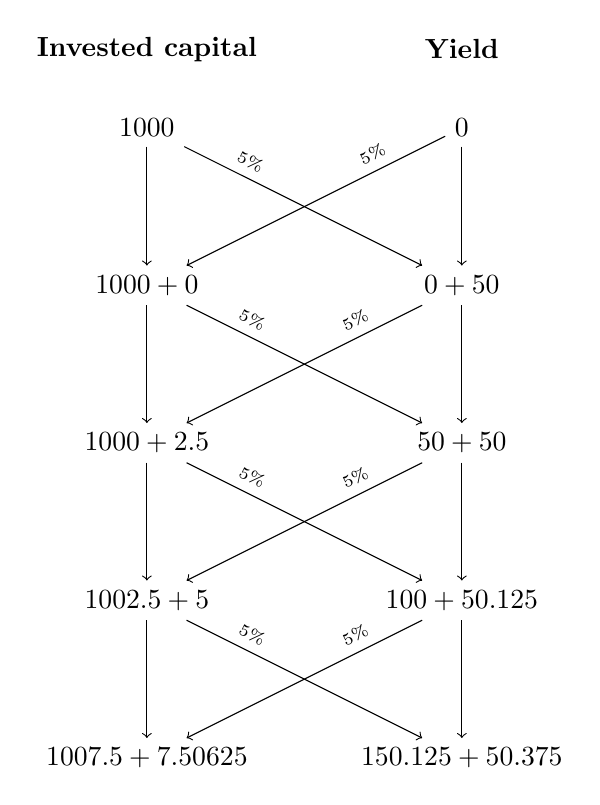
\begin{tikzpicture}
        \path (-2, 1)  node[fill=white, align=center]     {\textbf{Invested capital}};
        \path (2, 1)   node[fill=white, align=center]     {\textbf{Yield}};
        \path (-2, 0)  node[fill=white, align=center](x1) {1000};
        \path (2, 0)   node[fill=white, align=center](y1) {0};
        \path (-2, -2) node[fill=white, align=center](x2) {\(1000 + 0\)};
        \path (2, -2)  node[fill=white, align=center](y2) {\(0 + 50\)};
        \path (-2, -4) node[fill=white, align=center](x3) {\(1000 + 2.5\)};
        \path (2, -4)  node[fill=white, align=center](y3) {\(50 + 50\)};
        \path (-2, -6) node[fill=white, align=center](x4) {\(1002.5 + 5\)};
        \path (2, -6)  node[fill=white, align=center](y4) {\(100 + 50.125\)};
        \path (-2, -8) node[fill=white, align=center](x5) {\(1007.5 + 7.50625\)};
        \path (2, -8)  node[fill=white, align=center](y5) {\(150.125 + 50.375\)};
        
        \draw[->] (x1) -- (x2);
        \draw[->] (x2) -- (x3);
        \draw[->] (x3) -- (x4);
        \draw[->] (x4) -- (x5);
        
        \draw[->] (y1) -- (y2);
        \draw[->] (y2) -- (y3);
        \draw[->] (y3) -- (y4);
        \draw[->] (y4) -- (y5);
        
        \draw[->] (x1) -- node[near start, sloped, above] {\footnotesize{\(_{5\%}\)}} (y2);
        \draw[->] (x2) -- node[near start, sloped, above] {\footnotesize{\(_{5\%}\)}} (y3);
        \draw[->] (x3) -- node[near start, sloped, above] {\footnotesize{\(_{5\%}\)}} (y4);
        \draw[->] (x4) -- node[near start, sloped, above] {\footnotesize{\(_{5\%}\)}} (y5);
        \draw[->] (y1) -- node[near start, sloped, above] {\footnotesize{\(_{5\%}\)}} (x2);
        \draw[->] (y2) -- node[near start, sloped, above] {\footnotesize{\(_{5\%}\)}} (x3);
        \draw[->] (y3) -- node[near start, sloped, above] {\footnotesize{\(_{5\%}\)}} (x4);
        \draw[->] (y4) -- node[near start, sloped, above] {\footnotesize{\(_{5\%}\)}} (x5);
    \end{tikzpicture}
    \caption{Caption}
    \label{fig:compounding_example}
\end{figure}
Two approaches will be discussed that elegantly capture this process from a computational standpoint:  discrete LTI systems and hyperbolic-complex numbers. These methods are also closely related and essentially represent two sides of the same coin. The results that follow should therefore not come as surprising, though looking at them from different perspectives is certainly instructive.

\begin{figure}
    \centering
    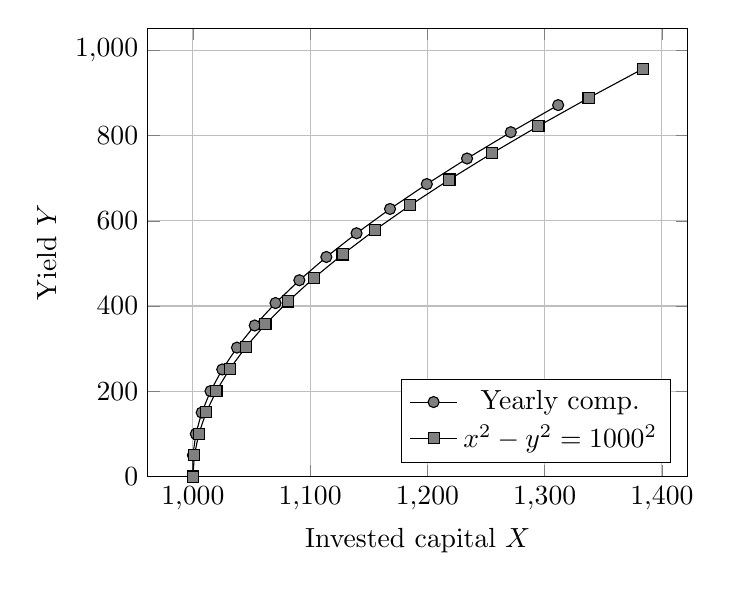
\begin{tikzpicture}[scale=1]
    \begin{axis}[
        xlabel={Invested capital $X$},
        ylabel={Yield $Y$},
        grid,
        cycle list name= black white,
        legend pos = south east,
        ymin = 0,
    ]
        \addplot coordinates {
                    (1000   ,  0     )
                    (1000   ,  50     )
                    (1002.5,  100    )
                    (1007.5,  150.125)
                    (1015.01,  200.5 )
                    (1025.03,  251.25)
                    (1037.59,  302.502)
                    (1052.72,  354.382)
                    (1070.44,  407.018)
                    (1090.79,  460.539)
                    (1113.82,  515.079)
                    (1139.57,  570.77)
                    (1168.11,  627.748)
                    (1199.5,  686.154)
                    (1233.8,  746.128)
                    (1271.11,  807.818)
                    (1311.5,  871.374)
                    % (135.507,  93.6949)
                    % (140.192,  100.47)
                    % (145.215,  107.48)
        };
        \addlegendentry{Yearly comp.};
        
        \addplot coordinates {
            (1000., 0.0)
            (1001.2502604383691, 50.020835937655015)
            (1005.0041680558036, 100.16675001984403)
            (1011.2711095766704, 150.56313315161269)
            (1020.0667556190758, 201.336002541094)
            (1031.4130998795731, 252.6123168081683)
            (1045.3385141288605, 304.52029344714266)
            (1061.8778191559855, 357.18972943727195)
            (1081.0723718384547, 410.7523258028155)
            (1102.970168555971, 465.34201693419774)
            (1127.6259652063807, 521.0953054937474)
            (1155.101414123941, 578.1516037434543)
            (1185.4652182422679, 636.6535821482414)
            (1218.793302887456, 696.7475261264401)
            (1255.169005630943, 758.5837018395335)
            (1294.6832846768447, 822.3167319358299)
            (1337.4349463048446, 888.1059821876231)
            (1383.530891937359, 956.1159599886322)
            %(143.30863854487743, 102.65167257081754)
            %(148.62253413851738, 109.94843179306726)
            %(154.30806348152436, 117.52011936438014)
        };
        \addlegendentry{$x^2 - y^2 = 1000^2$};
        
    \end{axis}
\end{tikzpicture}

    \caption{blabla}
    \label{fig:my_label}
\end{figure}